\documentclass[10pt]{article}

\usepackage[margin=0.75in]{geometry}
\usepackage{amsmath,amsthm,amssymb,bm}
\usepackage{xcolor}
\usepackage{cancel}
\usepackage{graphicx}
\usepackage{changepage}
\usepackage{circuitikz}
\usepackage{pgfplots}
\usepackage{minted}
\usepackage{physics}
\usepackage{tikz}
\usepackage{tikz-3dplot}
\usepackage{hyperref}
\usepackage{siunitx}
\usepackage{fontspec}
\usepackage{relsize}
\usepackage{subfig}
\usepackage{todonotes}
\usepackage{contour}
\usepackage{multicol, multirow, booktabs}
\usepackage[breakable]{tcolorbox}
\usepackage[inline]{enumitem}

\theoremstyle{definition}
\newtheorem{problem}{Problem}
\newtheorem{soln}{Solution}

\pgfplotsset{compat=newest}
\usetikzlibrary{lindenmayersystems}
\usetikzlibrary{arrows}
\usetikzlibrary{calc}
\usetikzlibrary{positioning, fit}
\usetikzlibrary{3d, perspective}
\usetikzlibrary{math}
\usetikzlibrary{fadings}
\usetikzlibrary{angles,quotes} 

\definecolor{incolor}{HTML}{303F9F}
\definecolor{outcolor}{HTML}{D84315}
\definecolor{cellborder}{HTML}{CFCFCF}
\definecolor{cellbackground}{HTML}{F7F7F7}
\newcommand{\ui}{\hat{i}}
\newcommand{\uj}{\hat{j}}
\newcommand{\uk}{\hat{k}}
\newcommand{\ux}{\hat{\mathbf{x}}}
\newcommand{\uy}{\hat{\mathbf{y}}}
\newcommand{\uz}{\hat{\mathbf{z}}}
\newcommand{\uv}[1]{\hat{\bv{{#1}}}}
\newcommand{\pr}[1]{{#1^\prime}}
\newcommand{\pd}[2][]{{\frac{\partial^{#1}}{\partial {{#2}^{#1}}}}}
\newcommand{\dif}[2][]{{\frac{d^{#1}}{d{{#2}^{#1}}}}}
\pgfdeclarelayer{background}  
\pgfsetlayers{background,main}
\AtBeginDocument{\RenewCommandCopy\qty\SI}

\makeatletter
\newcommand{\boxspacing}{\kern\kvtcb@left@rule\kern\kvtcb@boxsep}
\makeatother
\newcommand{\prompt}[4]{
    \ttfamily\llap{{\color{#2}[#3]:\hspace{3pt}#4}}\vspace{-\baselineskip}
}

\newcommand{\thevenin}[2]{
  \begin{center}
    \begin{circuitikz} \draw
      (0,0) -- (2,0) to[battery1, l_=$V_{Th}\eq#1$] (2,2) 
      to[resistor, l_=$R_{Th}\eq#2$] (0,2)
      ;
      \draw [o-] (-.07,2.079);
      \draw [o-] (-.07,0.079);
    \end{circuitikz}
  \end{center}
}

\newcommand{\norton}[2]{
  \begin{center}
    \begin{circuitikz} \draw
      (0,0) -- (3,0) to[american current source, l_=$I_{N}\eq#1$] (3,2) -- (0,2) (2,0)
      to[resistor, l=$R_{N}\eq#2$] (2,2)
      ;
      \draw [o-] (-.07,2.079);
      \draw [o-] (-.07,0.079);
    \end{circuitikz}
  \end{center}
}

\DeclareMathOperator{\Div}{div}
\DeclareMathOperator{\Curl}{curl}
\DeclareMathOperator{\sgn}{sgn}

\newcommand{\highlight}[1]{\colorbox{yellow}{$\displaystyle #1$}}

\newcommand{\ti}[1]{\widetilde{#1}}

\newfontface{\Kaufmann}{Kaufmann}
\DeclareTextFontCommand{\kf}{\Kaufmann}
\newcommand{\scriptr}{\fontsize{12pt}{12pt}\kf{r}}

\newfontface{\KaufmannB}{Kaufmann Bold}
\DeclareTextFontCommand{\kfb}{\KaufmannB}
\newcommand{\bscriptr}{\fontsize{12pt}{12pt}\kfb{r}}
\newcommand{\justif}[2]{&{#1}&\text{#2}}
\newcommand{\bv}[1]{\bm{\mathrm{#1}}}

\title{Physics 3200Y: Assignment VII}
\author{Jeremy Favro (0805980) \\ Trent University, Peterborough, ON, Canada}
\date{\today}

\begin{document}
\maketitle

% PROBLEM 1
\begin{problem}
Consider a current density $\bv{J}$ that in some region of space has the form $J_0y^2\ux$. Consider a surface that is made
from a section of cylinder, with its axis parallel to the $\uz$ direction and with radius $R$. Assume the surface extends
from $-L/2$ to $L/2$ along the $\uz$-direction, and from $\phi_1$ to $\phi_2$ in the angular direction. Find the current $I$ through
the surface in the following steps. Show your work, including integrals, explicitly:
\begin{enumerate}[label=(\alph*)]
  \item Draw a meaningful picture that I can read.
  \item Explain how you will parameterize your surface. Find the vector area element in terms of these parameters.
  \item Find the current through the surface. Do the integrals by hand and show your work.
\end{enumerate}
\end{problem}
\begin{soln}~
  \begin{enumerate}[label=(\alph*)]
    \item ~\tdplotsetmaincoords{60}{110}
          \begin{center}
            \begin{tikzpicture}[tdplot_main_coords]
              \colorlet{veccol}{green!50!black}
              \colorlet{projcol}{blue!70!black}
              \colorlet{myblue}{blue!80!black}
              \colorlet{myred}{red!90!black}
              \colorlet{mydarkblue}{blue!50!black}
              \tikzset{>=latex} % for LaTeX arrow head
              \tikzstyle{proj}=[projcol!80,line width=0.2, dashed] %very thin
              \tikzstyle{area}=[draw=veccol,fill=veccol!80,fill opacity=0.6]
              \tikzstyle{vector}=[-stealth,myred,thick,line cap=round]
              \tikzstyle{unit vector}=[->,veccol,thick,line cap=round]
              \tikzstyle{dark unit vector}=[unit vector,veccol!70!black]
              \usetikzlibrary{angles,quotes} % for pic (angle labels)


              % CONSTANTS
              \def\mrvec{4}
              \def\rvec{2}
              \def\phivec{10}
              \def\dz{3}
              \def\dphi{65}

              \coordinate (O) at (0,0,0);
              \draw[thick,->] (0,0,0) -- (\mrvec,0,0) node[anchor=north east]{$x$};
              \draw[thick,->] (0,0,0) -- (0,\mrvec,0) node[anchor=north west]{$y$};
              \draw[thick,->] (0,0,0) -- (0,0,\mrvec) node[anchor=south]{$z$};

              \foreach \y in {-6,...,6}{
                  \foreach \z in {-3,...,3}{
                      \tikzmath{
                        if \y != 0 then {
                            { \draw[vector] (-\y*\y/36, \y/6, \z) -- (\y*\y/36, \y/6, \z); };
                          };
                      }
                    }

                }

              \tdplotsetcoord{P1}{\rvec}{90}{\phivec} % s,theta,phi (rad, polar, azimuth)
              \draw[->, proj] (O) -- (P1xy) node [left] {\contour{white}{$\phi_1$}};
              \tdplotsetcoord{P2}{\rvec}{90}{\phivec + \dphi}
              \draw[->, proj] (O) -- (P2xy);

              \draw[area]
              plot[domain=0:.99*\dphi]({\rvec*cos(\phivec+\x)},{\rvec*sin(\phivec+\x)},{-\dz}) --
              plot[domain=-.99*\dz:.99*\dz]({\rvec*cos(\phivec+\dphi)},{\rvec*sin(\phivec+\dphi)},{\x}) --
              plot[domain=.99*\dphi:0]({\rvec*cos(\phivec+\x)},{\rvec*sin(\phivec+\x)},{\dz}) --
              plot[domain=.99*\dz:-.99*\dz]({\rvec*cos(\phivec)},{\rvec*sin(\phivec)},{\x}) --
              cycle;

              \draw[black, opacity=1, <->]
              ({(\rvec+0.1)*cos(\phivec+\dphi)},{(\rvec+0.1)*sin(\phivec+\dphi)},{-\dz})
              -- ({(\rvec+0.1)*cos(\phivec+\dphi)},{(\rvec+0.1)*sin(\phivec+\dphi)},{\dz})
              node [midway, right] {\contour{white}{$L$}};

              \foreach \y in {1,...,6}{
                  \foreach \z in {-3,...,3}{
                      \tikzmath{
                        if \y != 0 then {
                            { \draw[vector] (0, \y/6, \z) -- (\y*\y/36, \y/6, \z); };
                          };
                      }
                    }
                }
              \node[below left, proj] at (P2xy) {\contour{white}{$\phi_2$}};

              \node[vector] at (0, -1.4, 1) {$\bv{J}$};
            \end{tikzpicture}
          \end{center}
    \item I will parametrize the surface in terms of $\phi$ and $z$. Since the partial cylinder is of a fixed radius $R$, the area element is a small step in $\phi$ multiplied by $R$
          to create an arc-length along the surface, then
          times a small step in $z$, i.e. $d\bv{a}=Rd\phi dz\uv{s}$ since $\uv{s}$ is normal to the surface at all points.
    \item We know that
          $$\bv{J}=\frac{d\bv{I}}{da}$$ and so
          $$I=\int_\mathcal{S}\bv{J}\cdot d\bv{a}$$
          which in our case gives
          \begin{align*}
            I & =\int_\mathcal{S}J_0y^2\left[\cos\phi\uv{s}-\sin\phi\uv{\phi}\right]\cdot Rd\phi dz\uv{s}\justif{\quad}{Using coordinate transforms} \\
              & =RJ_0\int_{\phi_1}^{\phi_2}\int_{-L/2}^{L/2}R^2\sin^2\phi\cos\phi dzd \phi\justif{\quad}{Using coordinate transforms}                \\
              & =  R^3LJ_0\int_{\phi_1}^{\phi_2}\sin^2\phi\cos\phi  \phi \justif{\quad}{Pull out constant, no $z$ dependence}                        \\
              & =  R^3LJ_0\int_{\phi=\phi_1}^{\phi_2}u\,d u\justif{\quad}{$u=\sin\phi\implies \frac{du}{\cos\phi}=d\phi$}                            \\
              & =  R^3LJ_0\left[\sin^2\phi\right]_{\phi_1}^{\phi_2}\justif{\quad}{Undo substitution}                                                 \\
              & =  R^3LJ_0\left[\sin^2(\phi_2)-\sin^2(\phi_1)\right].
          \end{align*}
          Here the units of $J_0$ must be $\unit{\ampere\per\meter\tothe 4}$ for $J_0y^2$ to have units of $\unit{\ampere\per\meter\squared}$ as $\bv{J}$ was defined to have,
          and hence the units of the above expression are $\unit{\meter\cubed\meter\ampere\per\meter\tothe 4}=\unit{\ampere}$, which is comforting.
  \end{enumerate}
\end{soln}

% PROBLEM 2
\begin{problem}
Find, by direct integration of Eq. (5.16), the force on a circular loop of wire that lies in the $xy$ plane, has a
radius $R$, and carries a current $I$. The magnetic field is $\bv{B} = B_0(x-x_0)\uz$, where $B_0$ and $x_0$ are constants.
\begin{enumerate}[label=(\alph*)]
  \item Draw a meaningful picture that I can read.
  \item Explain how you will parameterize your line integral. Find the vector length element in terms of your
        parameters.
  \item Write explicit forms for the variables ($\bv{r}$, $\pr{\bv{r}}$, $\bscriptr$ etc.) you will need.
  \item Solve the integral by hand and show your work.
\end{enumerate}
\end{problem}
\begin{soln}
  \begin{enumerate}[label=(\alph*)]
    \item ~\tdplotsetmaincoords{60}{110}
          \begin{center}
            \begin{tikzpicture}[tdplot_main_coords]
              \colorlet{veccol}{green!50!black}
              \colorlet{projcol}{blue!70!black}
              \colorlet{myblue}{blue!80!black}
              \colorlet{myred}{red!90!black}
              \colorlet{mydarkblue}{blue!50!black}
              \tikzset{>=latex} % for LaTeX arrow head
              \tikzstyle{proj}=[projcol!80,line width=0.2, dashed] %very thin
              \tikzstyle{area}=[draw=veccol]
              \tikzstyle{vector}=[-stealth,myred,thick,line cap=round]
              \tikzstyle{unit vector}=[->,veccol,thick,line cap=round]
              \tikzstyle{dark unit vector}=[unit vector,veccol!70!black]
              \usetikzlibrary{angles,quotes} % for pic (angle labels)


              % CONSTANTS
              \def\mrvec{4}
              \def\rvec{2}
              \def\phivec{45}
              \def\dz{0}
              \def\dphi{360}

              \foreach \x in {-1,...,-6}{
                  \draw[vector] (\x/3, 0, -\x/3) -- (\x/3, 0, \x/3);
                }

              \coordinate (O) at (0,0,0);
              \draw[thick,->] (0,0,0) -- (\mrvec,0,0) node[anchor=north east]{$x$};
              \draw[thick,->] (0,0,0) -- (0,\mrvec,0) node[anchor=north west]{$y$};
              \draw[thick,->] (0,0,0) -- (0,0,\mrvec) node[anchor=south]{$z$};

              \foreach \x in {1,...,6}{
                  \draw[vector] (\x/3, 0, -\x/3) -- (\x/3, 0, \x/3);
                }

              \draw[area, ->]
              plot[smooth, domain=0:1.01*\dphi]({\rvec*cos(\phivec+\x)},{\rvec*sin(\phivec+\x)},{\dz});
              \node[below, green!50!black] at ({\rvec*cos(\phivec)},{\rvec*sin(\phivec)},{\dz}) {$I$};



              \node[vector] at (0, -1.4, 1) {$\bv{B}$};
            \end{tikzpicture}
          \end{center}
          Note that I've drawn this with $x_0=0$ though it does not have to be this way. Changing $x_0$ would shift where the field's sign changes.
    \item Here we need only one parameter as the curve is of fixed radius. I will call this $\phi$. This means that when we step through $d\phi$ we have travelled around the circle
          an (arc-)length $Rd\phi$ in the $\uv{\phi}$ direction.
    \item I don't think we can take the cross product directly in coordinate systems where the basis vectors change with position so we will need to convert everything
          to cartesian before we proceed (if I am wrong here it's no harm so long as I do the coordinate transforms right). The only thing we need to convert to cartesian coordinates
          is our length element. Borrowing from the back cover of Griffiths',
          $$d\bv{l}=Rd\phi\uv{\phi}=Rd\phi\left(-\sin\phi\ux+\cos\phi\uy\right).$$
    \item Equation (5.16) says that
          $$\bv{F}_{mag}=\int I \left(d\bv{l}\times \bv{B}\right)$$
          and so we compute the cross product first,
          $$
            d\bv{l}\times \bv{B}=\begin{vmatrix}
              \ux              & \uy             & \uz        \\
              -R\sin\phi d\phi & R\cos\phi d\phi & 0          \\
              0                & 0               & B_0(x-x_0)
            \end{vmatrix}=
            \left[RB_0(x-x_0)\cos\phi\right]\ux-\left[-RB_0(x-x_0)\sin\phi d\phi\right]\uy+0\uz
          $$
          and so the integral becomes (because $I$ is constant)
          $$RB_0 I\int_{0}^{2\pi}  \left[(x-x_0)\cos\phi\right]\ux+\left[(x-x_0)\sin\phi\right]\uy d\phi.$$
          Now $x$ is not constant in $\phi$ so we have to write it as a function of $\phi$ to properly compute the integral. Thankfully this is again in the back cover of
          Griffiths, $x=R\cos\phi$, so
          \begin{align*}
            \bv{F}_{mag} & =RB_0 I\int_{0}^{2\pi}  \left[(R\cos\phi-x_0)\cos\phi\right]\ux+\left[(R\cos\phi-x_0)\sin\phi\right]\uy d\phi            \\
                         & =RB_0 I\int_{0}^{2\pi}  \left[R\cos^2\phi-x_0\cos\phi\right]\ux+\left[R\cos\phi\sin\phi-x_0\sin\phi\right]\uy d\phi      \\
                         & =RB_0 I\int_{0}^{2\pi}  R\cos^2\phi\ux-x_0\cos\phi\ux+R\cos\phi\sin\phi\uy-x_0\sin\phi\uy d\phi                          \\
                         & =RB_0 I\int_{0}^{2\pi}  R\left[\cos^2\phi\ux+\cos\phi\sin\phi\uy\right]-\left[x_0\cos\phi\ux+x_0\sin\phi\uy \right]d\phi
          \end{align*}
          The second term in the integral comes out to zero as it's the integral of trig functions over one period,
          \begin{align*}
            \bv{F}_{mag} & =R^2B_0 I\int_{0}^{2\pi}  \left[\cos^2\phi\ux+\cos\phi\sin\phi\uy\right]d\phi                                                                                                                    \\
                         & =R^2B_0 I  \left[\frac{1}{2}\int_{0}^{2\pi}1+\cos(2\phi) d\phi\ux+\int_{\phi=0}^{2\pi}u\,du\uy\right]\justif{\quad}{Trig identity for $\cos^2x$, $u=\sin\phi\implies \frac{du}{\cos\phi}=d\phi$} \\
                         & =R^2B_0 I  \left[\frac{2\pi}{2}\ux+\eval{sin^2\phi}_{0}^{2\pi}\uy\right]\justif{\quad}{Integral of trig over full interval is zero}                                                              \\
                         & =R^2B_0 I\pi\ux.
          \end{align*}
          Again we check to see if the units make sense. To satisfy the definition of the magnetic field $B_0$ must have units of
          $\unit{\tesla\per\meter}=\unit{\kilo\gram\per\meter\per\ampere\per\second\squared}$ and so the above expression has units of
          $\unit{\meter\squared\ampere\kilo\gram\per\meter\per\ampere\per\second\squared}=\unit{\kilo\gram\meter\per\second}=\unit{\newton}$ which is comforting.
  \end{enumerate}
\end{soln}

% PROBLEM 3
\begin{problem}
Let there be an infinitely long hollow cylinder of radius $R$. The cylinder is conducting and carries surface current
density $\bv{K}$. The current has the form
$$\bv{K}=K_\phi\uv{\phi}+K_z\uv{z},$$
where $K_\phi$ and $K_z$ are constants. Find the magnetic field at a point along the central axis of the cylinder by
directly integrating Eq. (5.42) from the textbook.
\begin{enumerate}[label=(\alph*)]
  \item Draw a meaningful picture that I can read.
  \item Explain how you will parameterize your surface.
  \item Write explicit forms for the variables ($\bv{r}$, $\pr{\bv{r}}$, $\bscriptr$ etc.) you will need.
  \item Solve the integral by hand and show your work.
\end{enumerate}
\end{problem}
\begin{soln}
  \begin{enumerate}[label=(\alph*)]
    \item ~\tdplotsetmaincoords{90}{90}
          \begin{center}
            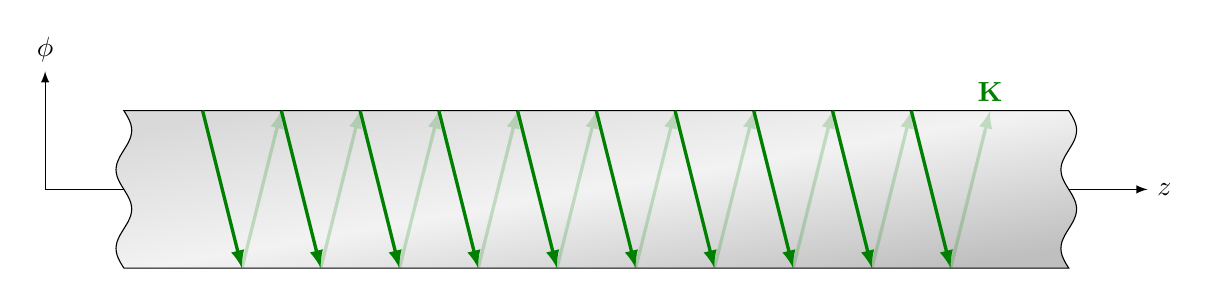
\begin{tikzpicture}
              \colorlet{veccol}{green!50!black}
              \colorlet{projcol}{blue!70!black}
              \colorlet{myblue}{blue!80!black}
              \colorlet{myred}{red!90!black}
              \colorlet{mydarkblue}{blue!50!black}
              \tikzset{>=latex} % for LaTeX arrow head
              \tikzstyle{proj}=[projcol!80,line width=0.2, dashed] %very thin
              \tikzstyle{area}=[draw=veccol,fill=veccol!80,fill opacity=0.6]
              \tikzstyle{vector}=[-stealth,myred,thick,line cap=round]
              \tikzstyle{unit vector}=[->,veccol,thick,line cap=round]
              \tikzstyle{dark unit vector}=[unit vector,veccol!70!black]
              \tikzstyle{metal}=[top color=black!15,bottom color=black!25,middle color=black!5,shading angle=10]


              % CONSTANTS
              \def\rvec{2}
              \def\lenvec{6}

              % Axes
              \draw[black,->] (-\lenvec-1,\rvec/2) -- (-\lenvec-1,\rvec+0.5) node[above]{$\phi$};
              \draw[black,->] (-\lenvec-1,\rvec/2) -- (\lenvec+1,\rvec/2) node[right]{$z$};

              % Cylinder
              \draw[metal] (-\lenvec,0) -- (\lenvec, 0) --
              plot[domain=0:\rvec, smooth]({\lenvec-0.1*sin(2*pi*\x r)}, {\x})
              -- (-\lenvec,\rvec) --
              plot[domain=\rvec:0, smooth]({-\lenvec-0.1*sin(2*pi*\x r)}, {\x});

              \def\w{1}
              \def\L{\lenvec}
              \def\R{\rvec}

              \foreach \i [evaluate={\x=-\L/2+(\i-1)*\w;}] in {-1,...,8}{
                  \draw[veccol, very thick, ->] (\x,\R)-- ({\x+\w/2},0);
                  \begin{scope}[transparency group, opacity=0.2]
                    \draw[veccol, very thick, ->] ({\x+\w/2},0)-- ({\x+\w},\R);
                  \end{scope}
                }
              \node[veccol] at (\lenvec-1, \rvec+0.235) {$\bv{K}$};

            \end{tikzpicture}
          \end{center}
    \item I will parametrize in terms of $z$ and $\phi$ with fixed $s=R$ with $z$ running from $-\infty$ to $\infty$ and $\phi$ from $0$ to $2\pi$ to sweep out the entire
          surface of the cylinder.
    \item Since the integral mentioned in the question is
          $$\bv{B}(\bv{r})=\frac{\mu_0}{4\pi}\int\frac{\bv{K}(\bv{r}')\times \bscriptr}{\scriptr^3}d\pr{a}$$
          we need $\bv{r}$, $\bv{r}'$, and $\bscriptr$. Since we are only looking at points on the axis of the cylinder $\bv{r}=(0,0,z)$ and
          $\bv{r}'=(x',y',z')$ which in terms of our parametrization variables is $\bv{r}'=(R\cos\phi',R\sin\phi',z')$ and hence
          $\bscriptr=\bv{r}-\bv{r}'=(-R\cos\phi',R\sin\phi',z-z')\implies \scriptr=\sqrt{R^2+(z-z')^2}$. To do the cross product we also have to rewrite $\bv{K}$
          in cartesian coordinates, $\bv{K}=K_\phi(-\sin\phi'\ux+\cos\phi'\uy)+K_z\uz$.
    \item The cross product in the integral becomes
          \begin{align*}
            \bv{K}(\bv{r}')\times \bscriptr & =\begin{vmatrix}
                                                 \ux              & \uy             & \uz    \\
                                                 -K_\phi\sin\phi' & K_\phi\cos\phi' & K_z    \\
                                                 -R\cos\phi'      & -R\sin\phi'     & (z-z')
                                               \end{vmatrix}         \\
                                            & =\left[K_\phi(z-z')\cos\phi'+RK_z\sin\phi'\right]\ux
            -\left[-K_\phi(z-z')\sin\phi'+RK_z\cos\phi'\right]\uy
            +\left[RK_\phi\sin^2\phi'+RK_\phi\cos^2\phi'\right]\uz                                 \\
                                            & =\left[K_\phi(z-z')\cos\phi'+RK_z\sin\phi'\right]\ux
            +\left[K_\phi(z-z')\sin\phi'-RK_z\cos\phi'\right]\uy
            +RK_\phi\uz
          \end{align*}
          And hence the integral becomes
          $$\bv{B}(\bv{r})=\frac{\mu_0}{4\pi}\int_{-\infty}^{\infty}\int_0^{2\pi}\frac{\left[K_\phi(z-z')\cos\phi'+RK_z\sin\phi'\right]\ux
              +\left[K_\phi(z-z')\sin\phi'-RK_z\cos\phi'\right]\uy
              +RK_\phi\uz}{\left(R^2+(z-z')^2\right)^{3/2}}d\phi'dz'$$
          which splits up into three integrals for each component of the field:
          \begin{align*}
            I_1 & =\int_{-\infty}^{\infty}\int_0^{2\pi}\frac{K_\phi(z-z')\cos\phi'+RK_z\sin\phi'}{\left(R^2+(z-z')^2\right)^{3/2}}d\phi'dz'\ux                                             \\
                & =\int_{-\infty}^{\infty}\int_0^{2\pi}\frac{K_\phi(z-z')\cos\phi'}{\left(R^2+(z-z')^2\right)^{3/2}}d\phi'dz'\ux \justif{\quad}{Integral of trig over full period is zero} \\
                & =\int_{-\infty}^{\infty}\frac{K_\phi(z-z')}{\left(R^2+(z-z')^2\right)^{3/2}}dz'\int_0^{2\pi}\cos\phi'd\phi'\ux                                                           \\
                & =0\justif{\quad}{Integral of trig over full period is zero}
          \end{align*}
          and we obtain the same result for the integral in the $\uy$ direction. The only nonzero integral is the $\uz$ one,
          \begin{align*}
            \bv{B}(\bv{r}) & =\frac{\mu_0}{4\pi}\int_{-\infty}^{\infty}\int_0^{2\pi}\frac{RK_\phi}{\left(R^2+(z-z')^2\right)^{3/2}}d\phi'dz'\uz  \\
                           & =\frac{\mu_0RK_\phi}{2}\int_{-\infty}^{\infty}\frac{1}{\left(R^2+(z-z')^2\right)^{3/2}}dz'\uz                       \\
                           & =\frac{\mu_0RK_\phi}{2}\int_{-\pi/2}^{\pi/2}\frac{-R\sec^2\theta}{\left(R^2+R^2\tan^2\theta\right)^{3/2}}d\theta\uz
          \end{align*}
          Here $z-z'=R\tan\theta\implies z-R\tan\theta=z'\implies dz'=-R\sec^2\theta d\theta$ and the limits change to the asymptotes of $\tan\theta$,
          \begin{align*}
             & =\frac{\mu_0RK_\phi}{2}\int_{-\pi/2}^{\pi/2}\frac{-R\sec^2\theta}{\left(R^2+R^2\tan^2\theta\right)^{3/2}}d\theta\uz           \\
             & =-\frac{\mu_0K_\phi}{2R}\int_{-\pi/2}^{\pi/2}\frac{\sec^2\theta}{\left(1+\tan^2\theta\right)^{3/2}}d\theta\uz                 \\
             & =-\frac{\mu_0K_\phi}{2R}\int_{-\pi/2}^{\pi/2}\frac{\sec^2\theta}{\sec^3\theta}d\theta\uz\justif{\quad}{$1+\tan^2 x=\sec^2 x$} \\
             & =-\frac{\mu_0K_\phi}{2R}\int_{-\pi/2}^{\pi/2}\cos\theta d\theta\uz\justif{\quad}{$\sec\theta=1/\cos\theta$} \\
             & =-\frac{\mu_0K_\phi}{2R}\left[\sin\frac{\pi}{2}+\sin\frac{\pi}{2}\right]\uz \\
             & =-\frac{\mu_0K_\phi}{R}\uz \\
          \end{align*}
          Let's check units: The units of $\mu_0$ are $\unit{\newton\per\ampere\squared}$ and the units of $K_\phi$ must be $\unit{\ampere\per\meter}$ to satisfy the
          definition of a surface current. Hence the units of the expression are $\unit{\newton\per\ampere\per\meter\squared}=\unit{\tesla\per\meter}$ which isn't right.
  \end{enumerate}
\end{soln}

% PROBLEM 4
\begin{problem}
A steady current $I$ flows down a long cylindrical wire of radius $a$. Find the magnetic field, both inside and outside the wire if:
\begin{enumerate}[label=(\alph*)]
  \item the current is uniformly distributed over the surface of the wire;
  \item the current is distributed in such a way that $J$ is proportional to $s$, the distance from the axis.
\end{enumerate}
\end{problem}
\begin{soln}
  \begin{enumerate}[label=(\alph*)]
    \item the current is uniformly distributed over the surface of the wire;
    \item the current is distributed in such a way that $J$ is proportional to $s$, the distance from the axis.
  \end{enumerate}
\end{soln}
\end{document}